\documentclass{article}

\usepackage{arxiv}

\usepackage[utf8]{inputenc} % allow utf-8 input
\usepackage{float}
\usepackage{listings}
\usepackage[T1]{fontenc}    % use 8-bit T1 fonts
\usepackage{hyperref}       % hyperlinks
\usepackage{url}            % simple URL typesetting
\usepackage{mathtools}
\usepackage{amssymb,mathrsfs}
\usepackage{booktabs}       % professional-quality tables
\usepackage{amsfonts}       % blackboard math symbols
\usepackage{ dsfont }
\usepackage{nicefrac}       % compact symbols for 1/2, etc.
\usepackage{microtype}      % microtypography
\usepackage{lipsum}		% Can be removed after putting your text content
\usepackage[spanish]{babel}


\title{El Problema del Agente Viajero usando la heurística de Aceptación por
Umbrales \emph{(Threshold Accepting)}}

%\date{September 9, 1985}	% Here you can change the date presented in the paper title
%\date{} 					% Or removing it

\author{
  Ángel Iván Gladín García\\
  No. cuenta: 313112470\\
  \texttt{angelgladin@ciencias.unam.mx} \\
}

% Uncomment to remove the date
%\date{}

% Uncomment to override  the `A preprint' in the header
%\renewcommand{\headeright}{Technical Report}
%\renewcommand{\undertitle}{Technical Report}

\begin{document}
\maketitle

\begin{abstract}
El Problema del Agente Viajero es un problema \emph{NP-Hard} que responde la siguiente pregunta;
``dada una lista de ciudades y las distancias entre cada par de ellas, ¿cuál es la ruta más corta
posible que visita cada ciudad exactamente una vez y al finalizar regresa a la ciudad origen?''

Que en su versión de optimización dice ``Dada una gráfica completa con pesos $G=(V,E)$, encontrar un ciclo
Hamiltonianto en $G$ con un peso mínimo (si acaso existe)''.

El método de Aceptación por Umbrales \emph{(Threshold Accepting)} es mucho más simple que Recocido
Simulado \emph{(Simmulated Annealing)} y es el motivo por el cual se usará para TSP.
\end{abstract}


\section{Introducción}
Para la resolución de TSP, primero se contruyó una gráfica $G=(V,E)$ con las ciudades y sus respectivas
distancias entre las ciudades con una base de datos que se nos fue dada. Esta gráfica ponderada
tiene una función de de peso para las aristas $w: E \to \mathds{R}^+$. Sea $S \subset V$ una
instancia de TSP que se quiera resolver.

Para hacer más sencillo la versión de optimización de este problema se hara uso de una
gráfica completa $G_s =(V_s, E_s)$, donde $V_s = S$ y $E_s= \{ (u,v) | u,v \in S \land u \not= v \}$,
con la función de peso amentada $w_s : E_s \to \mathds{R}^+$ definida como:
\[
  w_s(u,v) =
    \begin{cases}
      w(u,v)                   & \text{si }(u,v) \in E\\
      d(u,v) \times \max_d (S) &\text{e.o.c.}\\
    \end{cases}
\]

donde $d(u,v)$ es la distancia natural entre dos vértices $u$ y $v$; y $max_d (S)$ será la
distancia máxima de $S$.

La \textbf{distancia natural} se utiliza para calcular la distancia natural entre dos elementos
de $S$ para de esta manera tener nuestra gráfica completa, se utilizarán las coordenadas de las
ciudades correspondientes. Su fórmula está definida por
\[
    d(u,v) = R \times C
\]
donde $R$ es el radio de la Tierra y $C$ está definida como $C = 2 \times \arctan(\sqrt{A},\sqrt{1-A})$.

La \textbf{distancia máxima} de $S$ se define como:
\[
    \max_d (S) = \max \{ w(u,v) | u,s \in S \land (u,v) \in E \} 
\]

Una solución de TSP dada una instancia $S$, es cualquier permutación de de los elementos de $S$ y se
puede asegurar que estas soluciones son válidas para $G_s$. Dándonos así, dos tipos de permutaciones:
las factibles y las no factibles. Decimos que es factible si y sólo si las aristas entre dos elementos
consecutivos de la permutación existen en $E$. Si al menos una arista no existe, decimos que no es
factible.


La optimización de TSP necesitará una \textbf{función de costo} que evaluará ``qué tan buena (o no) es una
solución'' para así poder comparar burdamente las evaluación de ésta y así poder decidir cuál es
mejor utilizando el criterio de entre más \textit{pequeña} sea la evaluación es \textit{mejor}.
Para esto se va a normallizar la función de costo, pero para esto se necesitará un normalizador.

\textbf{El normalizador}, como su nombre lo dice, normalizar la función de costo y nos dirá si una
solución $S$ es factible si esta evaluada entre 0 y 1, y que una solución no factible se evalue con
un valor mayor que 1.

\textbf{Función de costo}, sea $S \subset V$ una instancia de TSP: la función de costo $f$ de una
permutación $P = v_{\rho(1)}, \ldots, v_{\rho(k)}$ de los elementos de $S$ está definida como:
\[
    f(P) = \frac{\sum_{i=2}^{k} w_s(v_{\rho(i-1)}, v_{\rho(i)})}{\mathcal{N}(S)}
\]

\section{Aceptación por Umbrales \emph{(Threshold Accepting)}}
Dado un problema $\mathscr{P}$ de optimización y clasificado como NP-duro, sea $S$ el conjunto de
posibles soluciones a una instancia de $\mathscr{P}$. Se supondrá que se tiene una función
$f: S \to \mathds{R}^+$, (función objetivo), tal que $0 \leq f(s) \leq \infty$ para cualquier
$s |in S$. Dadas $s,s'$ si $f(s) < f(s')$, entonces se considerará a la solición $s$ mejor que $s'$.

La idea central de \textbf{la aceptación por umbrales}, es dada una temperatura inicial
$T \in \mathds{R}^+$ y una solución inicial (obtenida de alguna manera). de forma aleatoria buscar
una solución vecina $s'$ tal que $f(s') \leq f(s) + T$, y entonces actualizar $s$ para que sea $s'$;
en este caso diremos que la solución $s'$ es \emph{aceptada}. Se continúa de esta manera mientras la
temperatura $T$ es disminuida paulatinamente siguiendo una serie de condiciones: el proceso termina
cuando $T < \epsilon$; cuando se han generado un determinado número de soluciones aceptadas; o
cuando otra serie de condiciones es satisfecha.

Para más detalles del algoritmo ver las notas de clase, que están situadas en \texttt{/spec}.

Citando\cite{DUECK1990161} el artículo,
\begin{quote}
  La diferencia escencial entre Simmulated Annealing y Threshold Accepting consiste de las diferentes
  reglas de aceptación. TA acepta \emph{cualquier} nueva configuración que no es mucho peor que la
  antigua (SA acepta peores soluciones solo con probabilidades bastante pequeñas).

  Una ventaja aparente de TA es una mayor simplicidad. No es necesario calcular las probabilidades
  o hacer una decisión aleatoria. Además se dice que:

  \begin{quotation}
    TA genera mejores resultados que SA (aunque en un considerable menor cantidad de tiempo
    respectivamente en una cantidad menor de ``nuevos pasos de elección de configuración'').
  \end{quotation}
\end{quote}

\section{Elaboración del programa}
Para ello, se escogió el lenguaje de programción \texttt{Kotlin} porque porque como requerimos
que sea un lenguaje compilado y que sea ``rápido''. Estoy utlizando Kotlin que se ejecuta sobre la
JVM. Además la sintaxis del lenguaje es moderna (comparado con Java) y me permite ser más expresivo
escribiendo menos, y la gran ventaja es que puedo utilizar todas las bibliotecas de Java.

Utilicé \texttt{Gradle} como sistema para la automatización de diferentes tareas, tales como la
de compilar, ejecutar y limpiar el proyecto. Su configuración es a través de DSL con el lenguaje
\texttt{Groovy}. Además permite la creación de \textit{tasks} de forma muy sencilla, por ejemplo
yo hice una \textit{task} para la creación de semillas, así puedo tener varias \textit{tasks} en el
proyecto de forma sencilla y solo indicado cual se quiere ejecutar.

Utilicé el IDE \texttt{IntelliJ IDEA}, porque me parece que tiene muchas herramientas, es rápido
y siempre da sugerencias útiles en el código y detecta errores de sintaxis muy rápido. Además
funciona muy bien con Kotlin.

Use \texttt{gnuplot} para gráficar las evaluaciones.

\section{Configuración del sistema}
Se pueden ver las constante que usaron para la configuración del sistema, situadas en\\
\texttt{src/main/kotlin/unam/ciencias/heuristicas/Constants.kt}, cabe notas que si se desean
modificar se debe volver a compilar el proyecto.

Se uso esta configuración:
\lstinputlisting[basicstyle=\small]{assets/code/tuning_constants.txt}


\section{Resultados}
Probando diferentes semillas de un lote de 500 semillas para ambas instancias de TSP (la de 40 y 150
ciudades), se logró encontrar una semilla para cada ejemplar de forma que se obtuviera una solución
``buena''. Para ello se generaron 500 semillas de forma aleatoria y se quedó con la que nos
diera una solución mejor.

\subsection{Instancia con 40 ciudades}
Con los identificadores de las ciudades:
\begin{verbatim}
  1,2,3,4,5,6,7,75,163,164,165,168,172,327,329,331,332,333,489,490,491,492,493,
  496,652,653,654,656,657,792,815,816,817,820,978,979,980,981,982,984  
\end{verbatim}

Usando la semilla \textbf{74440} nos da los siguientes resultados:
\begin{verbatim}
  Path: [652, 75, 792, 489, 817, 4, 165, 3, 333, 981, 6, 978, 5, 163, 172, 2, 656,
  653,490, 654, 820, 332, 982, 816, 7, 1, 168, 657, 815, 496, 329, 493, 979, 331,
  984, 491, 492, 164, 327, 980]
  Evaluation: 0.25787324528228406
  Feasible: true
\end{verbatim}

Graficando las evaluaciones con \texttt{gnuplot} se obtienen:
\begin{figure}[H]
  \centering
  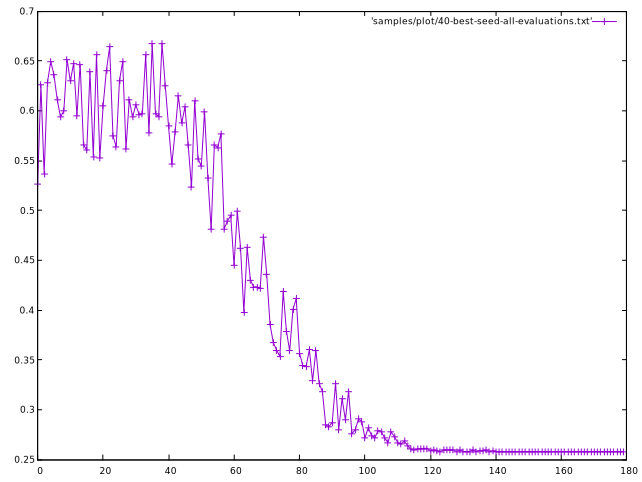
\includegraphics[scale=0.45]{assets/img/40-best-seed-all-evaluations.png}
  \caption{Mostrando todas las evaluaciones}
\end{figure}

\begin{figure}[H]
  \centering
  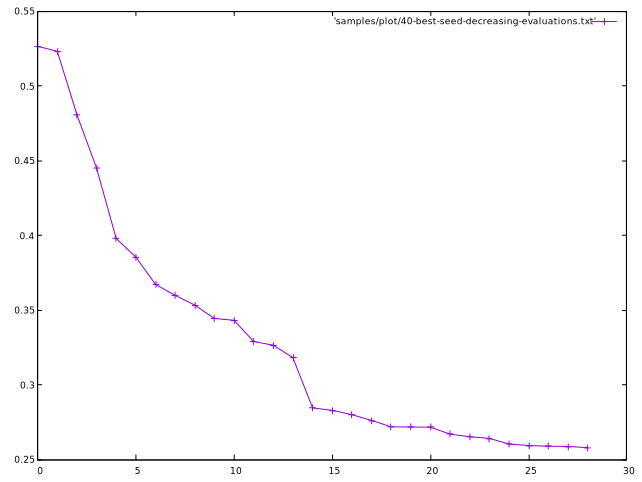
\includegraphics[scale=0.45]{assets/img/40-best-seed-decreasing-evaluations.png}
  \caption{Mostrando la mejora de cada evaluación}
\end{figure}

Y si visualizamos la ruta en un mapa, luce así:
\begin{figure}[H]
  \centering
  \includegraphics[width=\textwidth,height=\textheight,keepaspectratio]{assets/img/tps_best_40.png}
  \caption{Graficando la ruta usando el API de Google Maps}
\end{figure}


\subsection{Instancia con 150 ciudades}
Con los identificadores de las ciudades:
\begin{verbatim}
  1,2,3,4,5,6,7,8,9,11,12,14,16,17,19,20,22,23,25,26,27,74,75,77,163,164,165,166,
  167,168,169,171,172,173,174,176,179,181,182,183,184,185,186,187,297,326,327,328,
  329,330,331,332,333,334,336,339,340,343,344,345,346,347,349,350,351,352,353,444,
  483,489,490,491,492,493,494,495,496,499,500,501,502,504,505,507,508,509,510,511,
  512,520,652,653,654,655,656,657,658,660,661,662,663,665,666,667,668,670,671,673,
  674,675,676,678,792,815,816,817,818,819,820,821,822,823,825,826,828,829,832,837,
  839,840,978,979,980,981,982,984,985,986,988,990,991,995,999,1001,1003,1004,1037,
  1038,1073,1075
\end{verbatim}

Usando la semilla \textbf{30724} nos da los siguientes resultados:
\begin{verbatim}
  Path: [339, 186, 675, 1038, 12, 502, 340, 840, 350, 825, 500, 20, 660, 510, 343, 
  985, 674, 999, 8, 662, 331, 349, 1003, 11, 164, 501, 491, 499, 347, 817, 4, 174, 
  165, 988, 23, 176, 668, 352, 978, 6, 5, 1004, 981, 3, 333, 990, 353, 27, 991, 
  351, 185, 22, 676, 490, 654, 26, 820, 345, 332, 14, 181, 982, 187, 816, 678, 823, 
  7, 507, 653, 344, 665, 673, 184, 667, 656, 2, 173, 815, 9, 1, 829, 661, 832, 663, 
  657, 986, 508, 168, 505, 19, 496, 839, 182, 172, 163, 329, 509, 493, 979, 837, 
  995, 984, 826, 444, 17, 346, 792, 75, 821, 512, 179, 183, 77, 489, 25, 492, 334, 
  504, 327, 511, 670, 336, 980, 297, 1001, 822, 166, 1037, 494, 495, 167, 328, 326, 
  169, 1073, 330, 819, 655, 818, 666, 658, 74, 828, 520, 16, 671, 1075, 652, 483, 171]
  Evaluation: 0.16979788564331952
  Feasible: true

\end{verbatim}

Graficando las evaluaciones con \texttt{gnuplot} se obtienen:
\begin{figure}[H]
  \centering
  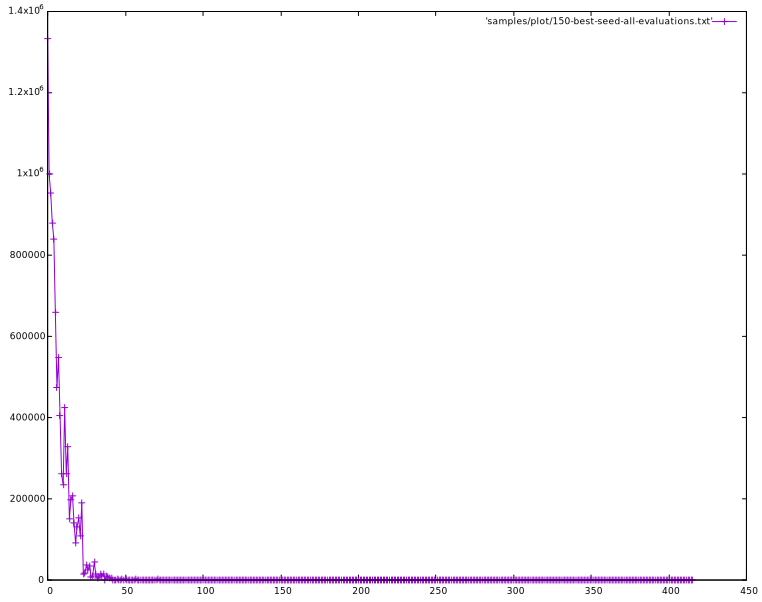
\includegraphics[scale=0.45]{assets/img/150-best-seed-all-evaluations.png}
  \caption{Mostrando todas las evaluaciones}
\end{figure}

\begin{figure}[H]
  \centering
  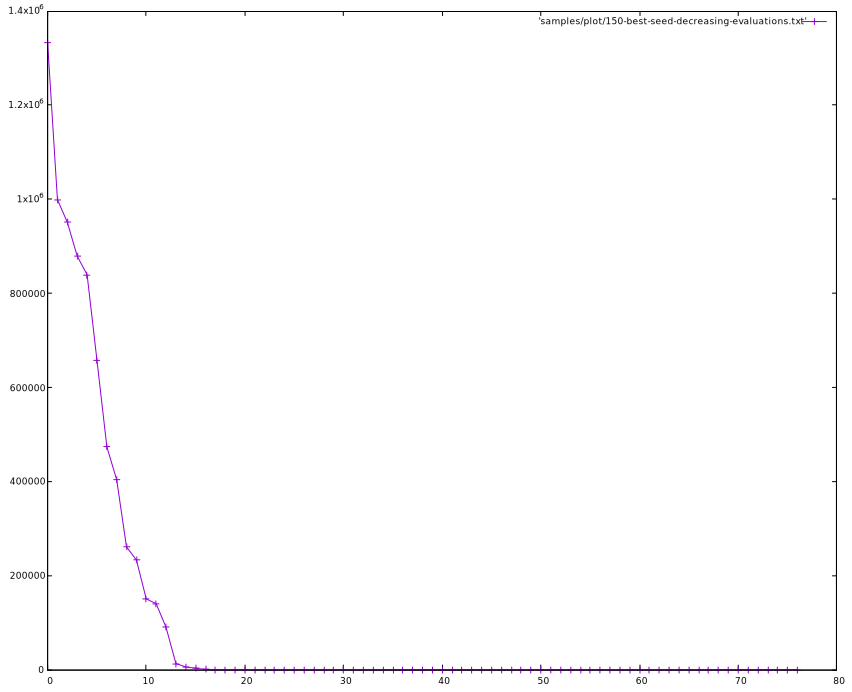
\includegraphics[scale=0.45]{assets/img/150-best-seed-decreasing-evaluations.png}
  \caption{Mostrando la mejora de cada evaluación}
\end{figure}

Y si visualizamos la ruta en un mapa, luce así:
\begin{figure}[H]
  \centering
  \includegraphics[width=\textwidth,height=\textheight,keepaspectratio]{assets/img/tsp_best_150.png}
  \caption{Graficando la ruta usando el API de Google Maps}
\end{figure}


\section{Comentarios}
En la elaboración y ejecución de este programa, me di cuenta lo importante que son las optimizaciones
de los algoritmos usados, aunque parezcan ser ``no tan importantes'', porque mejora su
tiempo significativamente.

También me hubiera gustado hacer el programa en \texttt{Rust} para así obtener una mejor
velocidad en la ejecución del programa.

Para ver como se ejecuta el programa y todo lo relacionado ver \texttt{README.md}

Se obtuvieron soluciones ``buenas'', pero no logré superar las del profesor sintiéndome así un tanto
enfadado conmigo.


\nocite{*}
\bibliographystyle{unsrt}  
\bibliography{references} 

\end{document}